% Appendix -- theory + reproducibility. Excluded from the 6-page limit.
\providecommand{\venuecompacttablefont}{\scriptsize}
% Source hygiene: omit private provenance identifiers from public builds.
\appendix

\section{SGCD Objective: Bounded Credit Reweighting}
\label{sec:theory}

We record the properties used in \S\ref{sec:method}. SGCD does not optimize a
standalone KL/JSD actor loss. Instead, it uses detached dense divergence
features to produce a bounded token-level multiplier on the policy-gradient
advantage. Let $j=(i,t)$ index a masked response token and let $A_i$ be the
trajectory-level group-relative advantage. Let
\[
  \begin{aligned}
  r_j(\theta)
  &=
  \frac{\pi_\theta(y_j\mid x_i,y_{i,<t})}
       {\pi_{\mathrm{old}}(y_j\mid x_i,y_{i,<t})},\\
  \bar r_j(\theta)
  &=
  \mathrm{clip}(r_j(\theta),1-\epsilon,1+\epsilon).
  \end{aligned}
\]
Reported runs use $\epsilon{=}0.2$ (bounds $[0.8,1.2]$).
The ordinary clipped GRPO token loss is
\[
  \ell_j^{\mathrm{GRPO}}(\theta)
  =
  -\min\{r_j(\theta)A_i,\bar r_j(\theta)A_i\}.
\]
SGCD computes detached credit features $u_j=\mathrm{sg}[d_j,H_j]$, where
$d_j$ is the dense teacher/student divergence and $H_j$ is teacher entropy.
The deterministic segmenter gives $s_j=g(u_j)$, and the bounded multiplier
satisfies $1\le W_j\le c$. In the reported implementation,
\[
  W_j=\mathrm{clip}(1+\gamma s_j,1,c),
\]
with $\gamma{=}1$ and $c{=}2$. The SGCD token loss is
\[
  \ell_j^{\mathrm{SGCD}}(\theta)
  =
  -\min\{r_j(\theta)A_iW_j,\bar r_j(\theta)A_iW_j\}.
\]
The propositions below concern this component; recipe-specific regularizers are
outside the notation.

\paragraph{Proposition 1 (no teacher-gradient path).}
Since $u_j$ is stop-gradient, $\partial W_j/\partial\theta=0$ for actor
parameters $\theta$. Therefore the SGCD credit-weighting path adds gradients
only through the reweighted policy ratio $r_j(\theta)$; it adds no
distillation-derived actor-gradient term of the form
\[
  \nabla_\theta D(\pi_\theta\Vert q_{\mathrm{teacher}}).
\]
Dense RKL and entropy are credit features, not a direct actor-gradient
distillation loss.

\paragraph{Proposition 2 (positive scaling of GRPO).}
For every token $j$,
\[
  \ell_j^{\mathrm{SGCD}}(\theta)
  =
  W_j\,\ell_j^{\mathrm{GRPO}}(\theta).
\]
Indeed, because $W_j>0$,
\[
  \min\{r_jA_iW_j,\bar r_jA_iW_j\}
  =
  W_j\min\{r_jA_i,\bar r_jA_i\}.
\]
Since $W_j$ is detached from actor parameters,
\[
  \nabla_\theta \ell_j^{\mathrm{SGCD}}(\theta)
  =
  W_j\nabla_\theta \ell_j^{\mathrm{GRPO}}(\theta).
\]
These equalities are pointwise where the clipped surrogate is differentiable;
at clip or minimum tie points, the same positive scaling holds for any
consistent subgradient choice because $W_j$ is detached and positive.

\paragraph{Corollary 1 (sign preservation).}
The reshaped advantage $\widehat A_j=A_iW_j$ satisfies
\[
  \mathrm{sign}(\widehat A_j)=\mathrm{sign}(A_i),
  \qquad
  |\widehat A_j|\le c|A_i|.
\]
Thus SGCD can scale local credit but cannot flip the sign of the
verifier-grounded advantage.

\paragraph{Corollary 2 (tokenwise PG alignment).}
For every token $j$,
\[
  \left\langle
  \nabla_\theta \ell_j^{\mathrm{SGCD}},
  \nabla_\theta \ell_j^{\mathrm{GRPO}}
  \right\rangle
  =
  W_j
  \left\|
  \nabla_\theta \ell_j^{\mathrm{GRPO}}
  \right\|^2
  \ge 0.
\]
Hence SGCD is tokenwise aligned with the corresponding GRPO update: it either
scales the same clipped-surrogate policy-gradient direction or, in a flat
clipped region, scales a zero gradient.

\paragraph{Corollary 3 (bounded contribution envelope).}
For every token,
\[
  \begin{aligned}
  |\ell_j^{\mathrm{SGCD}}|
  &\le c|\ell_j^{\mathrm{GRPO}}|,\\
  \|\nabla_\theta \ell_j^{\mathrm{SGCD}}\|
  &\le c\|\nabla_\theta \ell_j^{\mathrm{GRPO}}\|.
  \end{aligned}
\]
For a batch $B$,
\[
  \|\nabla_\theta L_{\mathrm{SGCD}}\|
  \le
  c\sum_{j\in B}
  \|\nabla_\theta \ell_j^{\mathrm{GRPO}}\|.
\]
This is a bound relative to the tokenwise policy-gradient contribution
envelope. It does not require, and does not imply, that SGCD's batch gradient is
within a factor $c$ of the realized GRPO batch gradient, because ordinary token
gradients may cancel and the bounded reweighting can change that cancellation.

\paragraph{Corollary 4 (bounded local movement under smooth KL).}
Assume the average policy KL is locally smooth, so that for sufficiently small
updates $\Delta\theta$,
\[
  \mathrm{KL}(\pi_\theta\Vert\pi_{\theta+\Delta\theta})
  \le
  \frac{L_{\mathrm{KL}}}{2}\|\Delta\theta\|^2 .
\]
For one SGCD step $\Delta\theta=-\eta\nabla_\theta L_{\mathrm{SGCD}}$,
\[
  \begin{aligned}
  &\mathrm{KL}(\pi_\theta\Vert\pi_{\theta+\Delta\theta})\\
  &\quad\le
  \frac{L_{\mathrm{KL}}}{2}
  \eta^2c^2
  \left(
  \sum_{j\in B}
  \|\nabla_\theta \ell_j^{\mathrm{GRPO}}\|
  \right)^2 .
  \end{aligned}
\]
This is not a global convergence or trust-region theorem. It states that SGCD's
policy movement is bounded by a clipped, detached reweighting of
verifier-grounded policy-gradient token contributions, rather than by an
independent teacher-matching actor loss.

\section{Reproducibility Details}
\label{sec:appendix}

\paragraph{Shared runtime configuration.} The AppWorld arms share the runtime
in Table~\ref{tab:recipe}, but only Vanilla GRPO uses reference-KL, with
coefficient $0.04$. The matched $\tau^3$-airline Vanilla GRPO and SGCD arms
share Table~\ref{tab:recipe_tau3}, including the same rollout, environment, and
evaluation harness, but only Vanilla GRPO uses reference-KL, with coefficient
$0.05$. The earlier SDPO collapse
run used a different diagnostic training recipe and is not covered by that
runtime table; its reported checkpoint was re-evaluated with the same canonical
held-out harness. The base student model is Qwen3.5-4B. These tables list shared
environment and sampling settings; method-specific hyperparameters are given in
\S\ref{sec:method} and \S\ref{sec:theory}.

\begin{table}[h]
  \centering
  \venuecompacttablefont
  \setlength{\tabcolsep}{3pt}
  \begin{tabular}{p{0.46\columnwidth}p{0.42\columnwidth}}
    \hline
    \textbf{Runtime setting} & \textbf{Value} \\
    \hline
    Base model                  & Qwen3.5-4B (raw) \\
    Rollouts per prompt ($n$)   & $8$ \\
    Train / mini-batch          & $8$ / $8$ \\
    PPO epochs                  & $1$ \\
    Learning rate               & $1\mathrm{e}{-6}$ \\
    Max prompt / response       & $16{,}384$ / $16{,}384$ tokens \\
    Max model length            & $32{,}768$ tokens \\
    Max user / assistant turns  & $30$ / $30$ \\
    Max observation             & $12{,}000$ chars \\
    Env steps per task          & $30$ \\
    Thinking enabled            & yes \\
    Rollout temp. / top-$p$ (train) & $1.0$ / $1.0$ \\
    Rollout temp. / top-$p$ (val)   & $1.0$ / $0.95$ \\
    Decoding (eval)             & greedy \\
    GPUs / tensor parallel      & $8$ / $1$ \\
    RL train/dev subset; held-out eval & $90$ / $57$ tasks; \texttt{test\_normal} $168$ + \texttt{test\_challenge} $417$ \\
    \hline
  \end{tabular}
  \caption{Shared runtime and environment configuration for the AppWorld arms.
    SGCD and the comparators use matched rollout-generation hyperparameters,
    evaluation settings, and the same environment/evaluator; only Vanilla GRPO
    includes reference-KL. SGCD
    instead uses detached divergence and mixed-sibling credit construction;
    Vanilla GRPO does not use mixed-group filtering. The response budget of $16{,}384$ tokens
    is shared across up to $30$ assistant turns; observations are truncated at
    $12{,}000$ characters. The train/dev counts are the RL subset used in these
    arms, not benchmark-wide official split counts. Held-out evaluation uses
    \texttt{test\_normal} ($168$ tasks / $56$ scenarios) and
    \texttt{test\_challenge} ($417$ / $139$) separately.}
  \label{tab:recipe}
\end{table}

\paragraph{Dynamic-sampling exhaustion.} The reported AppWorld and
$\tau^3$-airline SGCD runs use the same rule. Each candidate prompt group
contains eight siblings. We retain only complete mixed groups, targeting eight
kept groups per optimizer update, and refill for at most ten generation batches.
All-success and all-failure groups are discarded. If the target is still unmet
at the cap, the optimizer update is skipped and training continues.

\paragraph{$\tau^3$-airline runtime.} The matched Vanilla GRPO and SGCD arms
share the runtime in Table~\ref{tab:recipe_tau3}. Unlike the AppWorld arms, the $\tau^3$ policy is
initialized from a supervised checkpoint, which the diagnosis tracks as the
PG-dominant control (\S\ref{sec:diagnosis}). The interaction is bounded to $16$
user/assistant turns, and each tool/user observation is truncated to $512$
characters.

\begin{table}[h]
  \centering
  \venuecompacttablefont
  \setlength{\tabcolsep}{3pt}
  \begin{tabular}{p{0.46\columnwidth}p{0.42\columnwidth}}
    \hline
    \textbf{Runtime setting} & \textbf{Value} \\
    \hline
    Base model                  & Qwen3.5-4B, SFT-initialized \\
    Rollouts per prompt ($n$)   & $8$ \\
    Train / mini-batch          & $8$ / $8$ \\
    PPO epochs                  & $1$ \\
    Learning rate               & $1\mathrm{e}{-6}$ \\
    Max prompt / response       & $16{,}384$ / $16{,}384$ tokens \\
    Max model length            & $32{,}768$ tokens \\
    Max user / assistant turns  & $16$ / $16$ \\
    Max chars / observation     & $512$ \\
    Thinking enabled            & yes \\
    Rollout temp. / top-$p$ (train) & $0.4$ / $0.95$ \\
    Rollout temp. / top-$p$ (val)   & $0.4$ / $0.95$ \\
    Decoding (eval)             & greedy; $3$ seeds $\times$ $4$ trials \\
    GPUs / tensor parallel      & $8$ / $1$ \\
    Domain / held-out split     & airline / 20 task specs \\
    \hline
  \end{tabular}
  \caption{Shared runtime and environment configuration for the matched
    $\tau^3$-airline Vanilla GRPO and SGCD arms. The policy is SFT-initialized;
    Vanilla GRPO uses frozen-SFT low-variance reference-KL with fixed coefficient
    $0.05$, whereas SGCD omits reference-KL and uses detached divergence for
    credit weighting. The SDPO diagnostic training recipe is excluded from this
    table.}
  \label{tab:recipe_tau3}
\end{table}

\paragraph{$\tau^3$-airline user simulator.} All $\tau^3$-airline experiments
use the same instruction-following user simulator across arms. It role-plays the
airline customer according to the task specification. The same user-simulator
model and configuration are shared by the
SFT data generation, the Vanilla GRPO anchor, the SDPO collapse runs, and SGCD, so
the comparison introduces no method-specific user-simulator configuration.

\paragraph{$\tau^3$-airline SFT data and training.} After task-success and
format/trace validation, we retained $9{,}195$ full multi-turn trajectories
generated deterministically by \sftteacherproviderphrase{} paired with the same
instruction-following user simulator. A task-level split assigned $7{,}927$
trajectories from 25 tasks to SFT training and $1{,}268$ trajectories from three
tasks to SFT validation; each trajectory was one unpacked example. We trained
Qwen3.5-4B with full-parameter cross-entropy, maximum sequence length $32{,}768$,
global batch size $8$ (micro-batch $1$ per GPU), and constant learning rate
$1\mathrm{e}{-5}$ without warmup. The run was configured for two epochs
($990$ optimizer updates per epoch; $1{,}980$ planned) and stopped after saving
checkpoint step $1{,}600$ (1.62 epochs). All RL arms use the intermediate
step-$800$ checkpoint (0.81 epoch), selected from the step-$600$--$800$
validation-loss trough and subsequent rollout checks. It reaches held-out mean
Pass$^1$ $0.438$ on the 20-task-specification split
(Table~\ref{tab:tau3}), establishing the tool-use floor that naive SDPO
subsequently collapses and that PG-dominant training preserves.

\paragraph{Evaluation protocol.} AppWorld is scored with the benchmark's
state-based evaluator, reporting TGC and SGC \emph{separately} for
\texttt{test\_normal} ($168$ tasks / $56$ scenarios) and
\texttt{test\_challenge} ($417$ / $139$) under greedy decoding. These headline
values are the official evaluator aggregates, not success fractions reconstructed
from integer counts. The splits are not combined; the earlier
\texttt{batch\_001} SFT diagnostic in
\S\ref{sec:sftdiag} is a separately labeled pooled subset. The
$\tau^3$-airline diagnosis uses 20 held-out
task specifications (13 state-changing action tasks, 4 information-only tasks,
1 transfer, 2 no-action tasks). Evaluation uses a paired grid of three evaluation seeds
and four greedy trials per seed, giving 12 replay episodes per task specification
and 240 replay episodes total. Table~\ref{tab:tau3} reports binary success
(final evaluator reward $\geq1.0$), macro-averaged across task specifications.
Equal 12-episode task counts make this identical to total successes divided by
240. The representative SGCD row is 148/240 overall, 70/156 on
state-changing-action tasks, and 45/48 on information-only tasks.
In our internal ledgers, \texttt{write\_req} denotes state-changing action
tasks and \texttt{read\_only} denotes information-only tasks.
The same user simulator (strong instruction-following) drives the customer side
for both training rollouts and held-out evaluation. The zero-tool-collapse audit
measures, per training step, the fraction of information-only successes that
invoke no tool and the mean number of tools per information-only success. This
historical success-conditioned audit is distinct from
Figure~\ref{fig:tau_training_diag}, whose top panel reports mean tool count over
all diagnostic rollouts.

\paragraph{pass$^k$ vs.\ pass@$k$ (formal definition).}
We follow the $\tau$-bench evaluation protocol \citep{taubench2024}. The two
metrics have \emph{opposite} monotonicity in $k$:
\begin{itemize}
  \item \textbf{pass@$k$} (standard code-generation convention): draw $k$
    independent rollouts; a task is solved if \emph{at least one} succeeds:
    \[
      \mathrm{pass@}k = \mathbb{E}\!\left[
        1 - \prod_{i=1}^{k}(1-s_i)
      \right],
    \]
    where $s_i\in\{0,1\}$ is the success indicator of rollout $i$. Higher $k$
    \emph{increases} pass@$k$ (more attempts $\Rightarrow$ higher chance of
    at least one success).
  \item \textbf{pass$^k$} ($\tau$-bench convention): draw $k$ independent
    rollouts; a task is solved only if \emph{all $k$} succeed:
    \[
      \mathrm{pass}^k = \mathbb{E}\!\left[
        \prod_{i=1}^{k} s_i
      \right].
    \]
    Higher $k$ \emph{decreases} pass$^k$ (more attempts $\Rightarrow$ stricter
    consistency requirement). pass$^k$ measures \emph{reliability}: can the
    agent solve the task \emph{every time}, not just once?
\end{itemize}
In Table~\ref{tab:tau3} and throughout this paper, held-out \textbf{mean
Pass$^1$} is the task macro-average defined above; equal 12-episode task counts
make it identical to the 240-episode binary micro-average. The $\tau$-bench authors
motivate pass$^k$ as a
reliability metric for deployed agents where consistency matters more than
best-of-$k$ luck \citep{taubench2024}.

\paragraph{Credit-reference construction.} For a mixed sibling group, the
external LLM receives the policy-visible task instruction, rollout-visible
sibling traces, and each sibling's binary verifier outcome after sanitization. If
the entire set fits within context, all siblings are shown. If it is too long,
we include the smaller outcome class and match it with the opposite class. When
there are more successes than failures, we prefer shorter successful siblings;
when there are more failures than successes, we prefer longer failed siblings.
This keeps concise solutions and informative failures while staying within the
external LLM context. The reference is rebuilt from the current on-policy
siblings each time the task is sampled; we do not use a persistent skill bank.
The credit reference is generated by \creditreferenceproviderphrase{}, prompted with the
structured credit-scoring template in Table~\ref{tab:credit_prompt}.
Table~\ref{tab:external_models} summarizes the external components used only at
training time.

\begin{table}[h]
  \centering
  \venuecompacttablefont
  \setlength{\tabcolsep}{3pt}
  \begin{tabular}{p{0.28\columnwidth}p{0.62\columnwidth}}
    \hline
    \textbf{Component} & \textbf{Operational description} \\
    \hline
    Credit-reference LLM &
      \creditreferenceproviderphrase{} used only during training. Input is the
      sanitized task instruction plus mixed sibling traces and verifier outcomes;
      output follows Table~\ref{tab:credit_prompt}. Decoding, timeout, retry,
      and call/token accounting are implementation metadata. \\
    SFT trajectory teacher &
      \sftteacherproviderphrase{} used before RL to generate retained
      successful supervised-initialization trajectories with the same user
      simulator. Failed trajectories are discarded and the teacher is absent
      from RL rollouts and deployment. \\
    $\tau^3$ user simulator &
      \simulatorproviderphrase{} and task-specification prompt template
      across SFT data generation, Vanilla GRPO diagnostics, SDPO diagnostics, SGCD training, and
      held-out evaluation. No method-specific simulator prompt changes. \\
    \hline
  \end{tabular}
  \caption{Training-time external components. They are absent from deployment:
    the final student receives only the clean task prompt.}
  \label{tab:external_models}
\end{table}

\begin{table*}[t]
  \centering
  \venuecompacttablefont
  \setlength{\tabcolsep}{4pt}
  \begin{tabular}{p{0.20\textwidth}p{0.72\textwidth}}
    \hline
    \textbf{Prompt block} & \textbf{Template content} \\
    \hline
    Role &
    You are a training-time credit analyst. Given one task and several
    policy-generated sibling rollouts with verifier outcomes, write a concise
    stepwise credit reference. \\
    Input &
    Task instruction; visible tool/API traces and observations for each
    sibling; each sibling's success/failure outcome; rollout-visible alignment
    metadata such as turn/order identifiers. \\
    Rules &
    Use only information present in the visible traces. Do not quote hidden
    labels, evaluator reports, credentials, or final answer literals. Prefer
    abstract state checks and action choices over copying task-specific values. \\
    Output &
    (1) state checks that successful siblings establish; (2) reusable
    successful action branches; (3) failed branches and why they appear wrong;
    (4) likely deviation points where failures depart from successful evidence;
    (5) literals or values that should remain masked during credit scoring. \\
    Use &
    Insert this reference only in the teacher-side scoring prefix during
    training. Never insert it into the student rollout prompt or deployment
    prompt. \\
    \hline
  \end{tabular}
  \caption{Credit-reference prompt template. The template is intentionally
    benchmark-generic: sibling traces provide the evidence, while the prompt
    asks the external LLM to abstract reusable state/action credit rather than
    copy hidden answers.}
  \label{tab:credit_prompt}
\end{table*}

\paragraph{Leakage and literal masking.} Before calling the external LLM, we
remove benchmark-private supervision and values that should not be recoverable
from the clean deployment prompt. Concretely, the sanitizer masks evaluator or
oracle reports, hidden gold actions, credentials, payment or account values,
and answer-bearing literals. This rule is not AppWorld-specific: for any
tool-use benchmark, the credit reference may summarize policy-visible behavior
and observations, but it may not expose private labels or task answers.

\paragraph{Dense credit features.} We project both the clean-student distribution
and the credit-reference-conditioned teacher distribution onto the same local
support containing the teacher top-$100$ tokens, the observed token, and a tail bucket.
The reported results use reverse-KL; no alternative-divergence ablation is
claimed. Divergence spikes and teacher
entropy define credit saliency before the bounded credit multiplier produces
token weights.

\paragraph{Credit segmenter.} SGCD uses a deterministic reverse-KL/entropy
segmenter with sibling-derived credit-reference teacher context rather than a
ground-truth-conditioned teacher. For each assistant response, let $d_{\min}$
and $d_{\max}$ denote the minimum and maximum dense reverse-KL. We normalize
$d_t$ as $\tilde d_t=(d_t-d_{\min})/(d_{\max}-d_{\min}+\epsilon_{\mathrm{norm}})$,
using $\epsilon_{\mathrm{norm}}=0.1$. A segment starts when
$\tilde d_t>\lambda_{\mathrm{KL}}=0.15$ and extends until either entropy exceeds
$\lambda_H=1.5$ times its onset value or its length reaches $0.2T$, where $T$ is
the rollout length. There is no additional minimum-length constraint. Tokens inside a triggered segment receive the
onset saliency; tokens outside triggered segments use their local
$\tilde d_t$. There is no learned saliency network. The final multiplier remains
bounded by Eq.~\ref{eq:weight_layer}, with $\gamma{=}1$ and $c{=}2$.

\paragraph{Response and credit masks.} Policy-gradient loss is computed only on
assistant-generated response tokens. System prompts, user/task prompts, API
documentation, tool observations, simulator returns, and the credit-reference
prefix itself are masked out. Generated reasoning tokens remain model output and
can receive the ordinary PG loss; SGCD may also use their detached divergence as
credit evidence. API/action spans are additionally logged as a safety and
analysis slice, but fixed tool-call boundaries are not the only credit segments.
Answer-bearing literals and masked values are excluded from credit-reference
scoring; for response tokens that remain in the policy-gradient mask, SGCD
saliency is zero and therefore $W=1$.

\paragraph{Runtime monitoring.} Dense teacher scoring adds an extra forward
path, so we monitor step time, dense-scoring time, selected dense-token counts,
credit-token counts, and peak GPU memory. The run is considered invalid if the
dense features are all zero, the credit weights are inert, response masks include
prompt/tool-observation tokens, or the detached divergence path becomes a direct
actor-gradient KL/JSD loss.

\section{Additional Result Tables}
\label{sec:appendix_tables}

The main body reports headline results (Tables~\ref{tab:appworld}--\ref{tab:tau3}),
the seed summary (Table~\ref{tab:seedrobust}), and the ablation grid
(Table~\ref{tab:ablation}). This section collects the
self-distillation method family comparison (Table~\ref{tab:sdfamily}) for
reference: it positions SGCD's use of distillation as detached credit features
rather than a standalone actor-gradient loss, the structural distinction from
prior SD methods.

\paragraph{Direct-SD diagnostic row.} The direct/uncapped SD row uses the same
credit-reference teacher context, top-$100$ local support, and assistant-response
mask as SGCD, but feeds the teacher/student divergence into a standalone
teacher-matching auxiliary of the form
$\mathcal{L}_{\mathrm{PG}}+\lambda\mathcal{L}_{\mathrm{SD}}$
rather than the bounded detached multiplier. It is the controlled, in-codebase
analogue of the SDPO-style direct self-distillation failure in \S\ref{sec:diagnosis}.
Relative to SGCD's ablation setting, the salient change is that the divergence
enters as an actor gradient instead of a detached credit weight. We report it as
a single untuned diagnostic setting with a lower point estimate than the reported
Vanilla GRPO, not as a swept baseline; we did not tune $\lambda$ or its
schedule. The archived run/evaluation ledger does not retain the numerical
coefficient or schedule, so this row should be interpreted only as a diagnostic
comparison and not as a fully reproducible baseline.


\begin{table*}[t]
  \centering
  \venuecompacttablefont
  \setlength{\tabcolsep}{4pt}
  \begin{tabular}{p{0.13\textwidth}p{0.23\textwidth}p{0.31\textwidth}p{0.21\textwidth}}
    \hline
    \textbf{Method} & \textbf{Objective role} & \textbf{Teacher / privileged context} & \textbf{Signal used} \\
    \hline
    SDPO \citep{sdpo2026}      & feedback-conditioned SD         & rich feedback / successful samples & sym.\ JSD or RKL; student-top-$K$ + tail \\
    OPSD \citep{opsd2026}      & standalone reward-free SD       & label-privileged trace / answer & full-vocab forward KL; JSD-$\beta$ ablated \\
    Skill-SD \citep{skillsd2026} & GRPO $+\lambda$ SD loss       & trajectory-derived NL skill summaries & imp.-weighted reverse-KL \\
    SDAR \citep{sdar2026}      & GRPO $+\lambda$ gated SD aux    & retrieved skill / privileged context & $\sigma(\beta\Delta)$ gap gate \\
    \textbf{SGCD (ours)}       & \textbf{PG credit reweighting}  & \textbf{mixed siblings summarized into a credit reference} & \textbf{dense RKL+entropy, detached credit weights} \\
    \hline
  \end{tabular}
  \caption{Self-distillation method family. SGCD uses distillation differently:
    teacher/student divergence is a detached credit-assignment signal for the
    policy-gradient surrogate, not a standalone actor-gradient auxiliary.}
  \label{tab:sdfamily}
\end{table*}

\section{Training-Trajectory Diagnostics}
\label{sec:training_trajectory_diagnostics}

The held-out tables in the main paper are the primary result. Figures
\ref{fig:tau_training_diag} and \ref{fig:appworld_training_diag} provide
training-trajectory diagnostics: the $\tau^3$ plot tracks tool-use behavior,
while the AppWorld plot tracks validation success and completion.

\begin{figure*}[t]
  \centering
  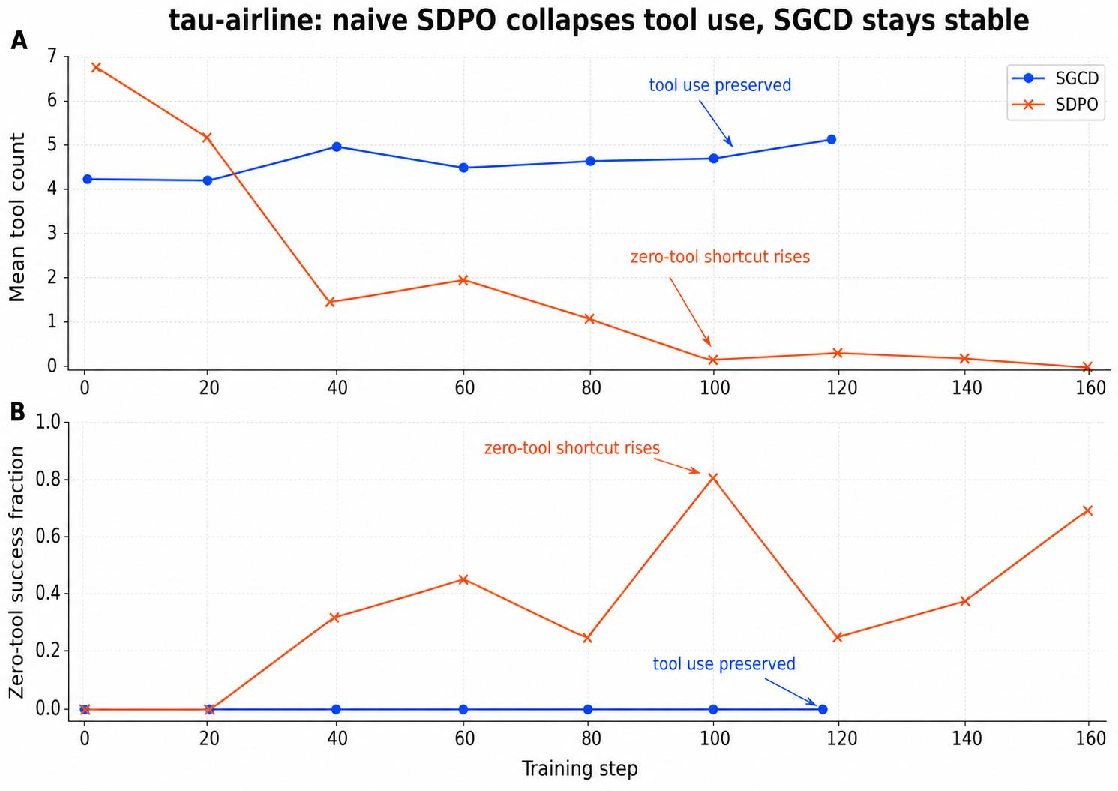
\includegraphics[width=0.96\textwidth]{f_appendix_tau_training_diag.pdf}
  \caption{$\tau^3$-airline training diagnostic trajectories. In this diagnostic
    trace, SDPO loses tool/action behavior during training, while the SGCD trace
    retains nonzero tool use and does not show the zero-tool fixed point. These training traces diagnose the
    training-time failure mode; Table~\ref{tab:tau3} reports the held-out
    mean Pass$^1$ comparison.}
  \label{fig:tau_training_diag}
\end{figure*}

\begin{figure*}[t]
  \centering
  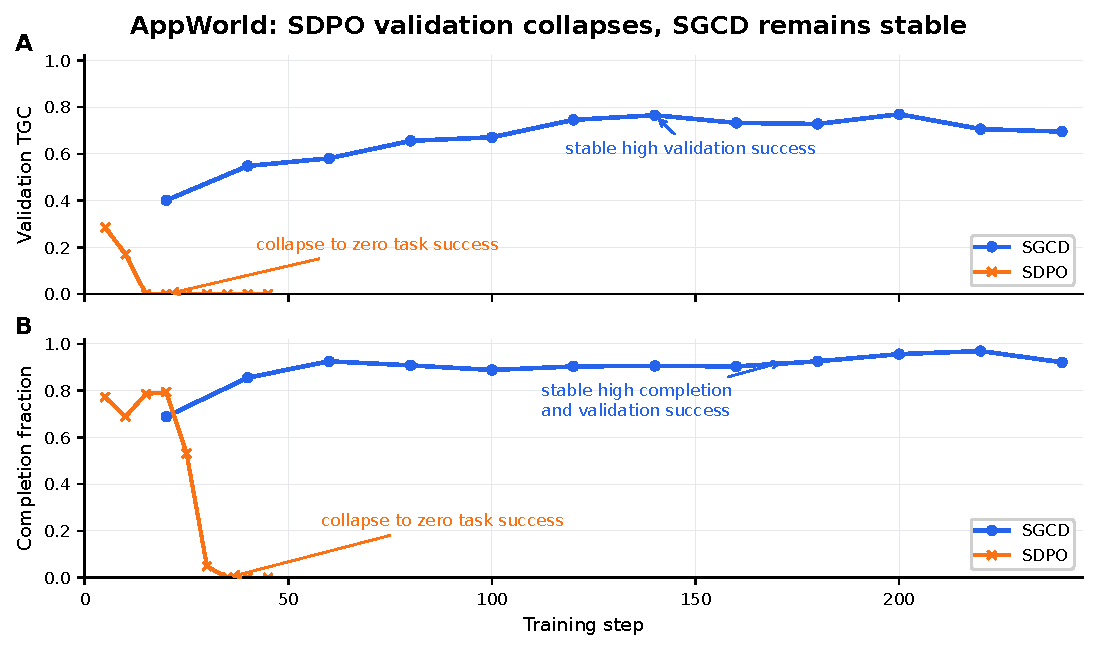
\includegraphics[width=0.96\textwidth]{f_appendix_appworld_training_diag.pdf}
  \caption{AppWorld training diagnostic trajectories. In the available diagnostic trace,
    SGCD maintains high validation and completion values through the 240-step run, while the SDPO diagnostic run
    collapses early in both task success and completion-related signals. The
    AppWorld SDPO curve stitches resumed diagnostic runs and is used as failure
    evidence, not as a replacement for the held-out result table. It is a
    separate training-trajectory diagnostic and is not numerically comparable
    to the held-out direct/uncapped ablation row in Table~\ref{tab:ablation}.}
  \label{fig:appworld_training_diag}
\end{figure*}

\FloatBarrier

\section{AppWorld SFT Diagnostic}
\label{sec:sftdiag}

Table~\ref{tab:appworld_sft_diag} summarizes the diagnostic AppWorld SFT ladder
that motivated direct-from-base RL for AppWorld. These runs used an early
\texttt{batch\_001} diagnostic subset, so they are not numerically comparable to
the held-out \texttt{test\_normal}/\texttt{test\_challenge} headline table. They
nevertheless show the qualitative issue: standard SFT reduced next-token loss
while sharply degrading executable AppWorld behavior.

\begin{table}[h]
  \centering
  \venuecompacttablefont
  \setlength{\tabcolsep}{3pt}
  \begin{tabular}{lccc}
    \hline
    \textbf{Run} & \textbf{Rows / traj.} & \textbf{TGC} & \textbf{Test-pass} \\
    \hline
    Base 4B       & -- & \textbf{15.8} & \textbf{51.5} \\
    SFT v0        & 770 turn rows & 1.1 & 17.7 \\
    SFT v0.5      & 4,288 turn rows & 0.6 & 15.3 \\
    SFT v0.6      & 393 trajectories & looping & -- \\
    \hline
  \end{tabular}
  \caption{Diagnostic AppWorld SFT regression on a pooled
    \texttt{test\_normal}+\texttt{test\_challenge} \texttt{batch\_001}
    subset (177 trajectories: 51 normal and 126 challenge; 1,363 executable
    unit tests). TGC counts are 28/177, 2/177, and 1/177 for Base 4B, SFT v0,
    and SFT v0.5; corresponding test-pass counts are 702/1,363, 241/1,363, and
    208/1,363. The result
    motivates starting AppWorld SGCD from the base 4B model, unlike the
    $\tau^3$-airline ladder where SFT is a viable initialization.}
  \label{tab:appworld_sft_diag}
\end{table}
